\chapter{BitMar: Low-Bit Multimodal Foundation for Edge Deployment}
\label{cha:bitmar}

This chapter presents BitMar~\cite{aman2025bitmar}, the first published contribution of this thesis research. BitMar is framed as a proof-of-concept and foundational work that established key design principles, notably the compatibility of extreme quantization with cross-modal fusion and episodic memory conditioning, which were later refined and scaled in the EmberVLM system (Chapter~\ref{cha:embervlm}).

\section{Motivation and Research Goals}
\label{sec:bitmar_motivation}

The design of BitMar is motivated by a specific question: \emph{Can a model with only 14 million parameters, operating under 1.58-bit ternary weight quantization, achieve meaningful multimodal understanding and generation while incorporating an external episodic memory?}

This question is non-trivial because each component introduces constraints on the others. Quantization reduces the information capacity per parameter, potentially limiting the model's ability to learn fine-grained cross-modal correspondences. Cross-modal fusion requires the text and vision representations to be sufficiently expressive to support accurate attention-based alignment despite the quantization noise. Episodic memory adds a fixed-overhead read/write mechanism that must integrate cleanly with the quantized decoder without introducing instability or gradient conflicts.

\paragraph{Why 1.58-bit?} Ternary weight quantization at 1.58 bits/parameter enables replacing floating-point multiply-accumulate operations with additions and subtractions. A ternary weight $w \in \{-1, 0, +1\}$ applied to activation $a$ gives: $w \cdot a \in \{-a, 0, +a\}$. This means every MHSA and FFN projection can be computed without a single floating-point multiplication, with only conditional negation or zeroing. On hardware without dedicated floating-point units, this is a substantial speedup. Even on standard CPUs, integer arithmetic is significantly faster than floating-point, making ternary quantization the preferred precision for the target edge hardware.

The three design goals for BitMar are:
\begin{enumerate}
    \item \textbf{Unified low-bit multimodal encoding}: both text and vision representation pathways operate under the same 1.58-bit quantization regime, ensuring consistent hardware efficiency across the entire model.
    \item \textbf{Cross-modal fusion under quantization constraints}: the fusion mechanism must preserve semantic alignment between modalities despite ternary weight projections, validated by a contrastive cross-modal alignment objective.
    \item \textbf{External episodic memory without parametric overhead}: the memory system must improve contextual coherence and task accuracy without significantly increasing the trainable parameter count, and must not require any additional inference hardware.
\end{enumerate}

\section{BitMar Architecture Overview}
\label{sec:bitmar_arch}

BitMar follows a four-stage pipeline, illustrated in Figure~\ref{fig:bitmar_arch}:
\begin{enumerate}
    \item \textbf{Parallel low-bit encoders}: A 1.58-bit BitNet-style text encoder and a DiNOv2-based vision encoder (with MLP compression) produce 128-dimensional representations of the input text and image respectively.
    \item \textbf{Cross-modal fusion}: A lightweight cross-attention module (text queries, vision keys/values) fuses the two modalities into a shared 128-dimensional representation.
    \item \textbf{Episodic memory conditioning}: The fused multimodal embedding queries a fixed-size episodic memory matrix ($K{=}512$, $C{=}128$), retrieving a context vector that conditions the decoder.
    \item \textbf{Memory-conditioned autoregressive decoding}: A 1.58-bit BitNet decoder generates text output, with per-layer conditioning from the retrieved memory vector.
\end{enumerate}

All trainable weight matrices in the text encoder, fusion module, and decoder use ternary weights $\{-1, 0, +1\}$ with learned per-layer scales. Activations use 8-bit quantization with per-token max-abs scaling. Softmax, residual connections, and layer normalization operate in FP32 to preserve numerical stability.

\begin{sidewaysfigure}[p]
    \centering
    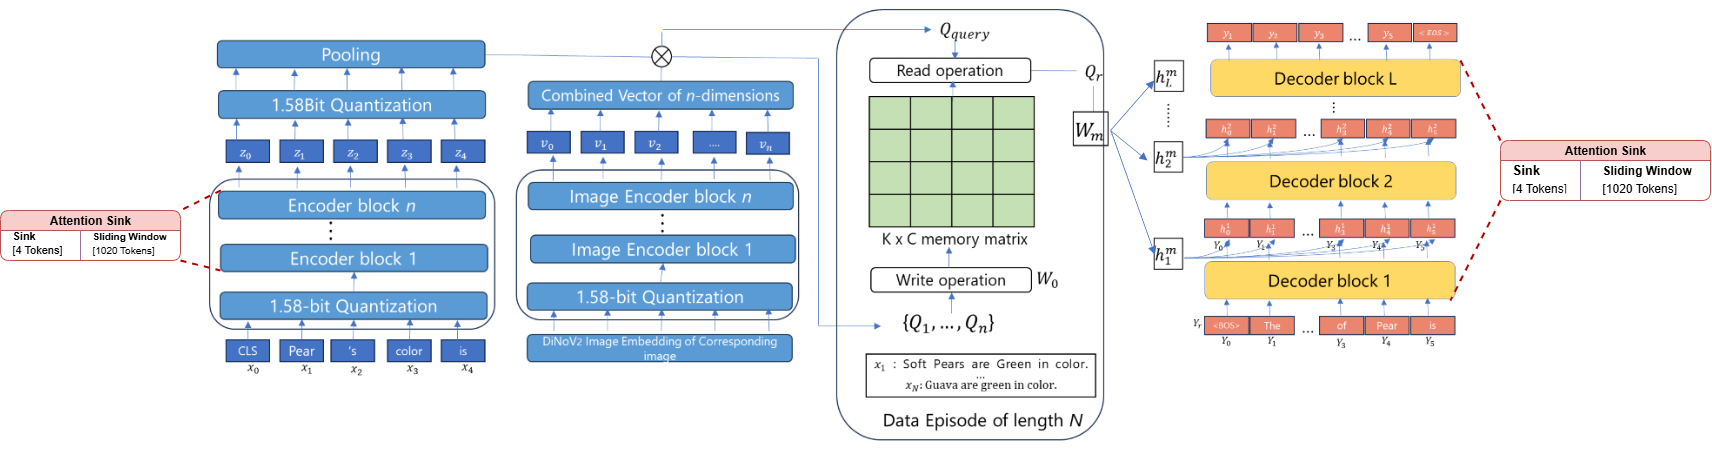
\includegraphics[width=\textheight]{../BabyLM_new/FIG/BitMar-Architecture.png}
    \caption{\textbf{BitMar Architecture.} The model processes multimodal inputs: text tokens and DiNOv2-compressed image features. Quantized encoders (1.58-bit) generate compact text and vision embeddings ($z$, $v$), which are fused via cross-modal attention into shared query representations. A sliding-window attention mechanism enables long-context processing. A fixed episodic memory matrix ($K \times C$) stores and retrieves multimodal context vectors through quantized read/write weights, supporting optional SD-card offloading for edge deployment.}
    \label{fig:bitmar_arch}
\end{sidewaysfigure}

\section{Text Encoder}
\label{sec:bitmar_text_encoder}

\subsection{Architecture}
The BitMar text encoder is a lightweight quantized Transformer with 4 layers, hidden dimension $d{=}128$, and $h{=}4$ attention heads, supporting sequences of up to 256 tokens.

\subsection{Quantization}
Two levels of quantization are applied:

\paragraph{Weight Quantization.} All linear projection weights in MHSA and FFN sublayers are quantized to ternary values $\{-1, 0, +1\}$ using learned per-layer scaling factors $\gamma$:
\begin{equation}
    \hat{W} = \mathrm{RoundClip}\!\left(\frac{W}{\gamma + \epsilon},\ -1,\ 1\right), \quad \gamma = \frac{1}{nm}\sum_{i,j}|W_{ij}|
\end{equation}
where $\mathrm{RoundClip}(\cdot, a, b) = \max(a, \min(b, \mathrm{round}(\cdot)))$ maps each weight to the nearest ternary value. The scale $\gamma$ is the mean absolute value of the unquantized weight matrix, trained jointly with the network parameters.

\paragraph{Activation Quantization.} Token-wise activations are quantized to 8 bits using per-token max-abs scaling:
\begin{equation}
    \hat{\mathbf{x}}_t = \mathrm{round}\!\left(\frac{\mathbf{x}_t}{\max_j |x_{t,j}|} \times 127\right)
\end{equation}
This localized scaling preserves fine-grained detail for each token by adapting to that token's specific activation range.

\subsection{Attention Sinks for Long-Context Processing}
Attention sinks are injected into every self-attention layer to enable efficient long-sequence processing. With $S{=}4$ persistent sink tokens and a sliding window of $W{=}1{,}020$, the KV cache maintains global context anchors alongside recent tokens. When a new token arrives, the oldest window token is evicted, sink and window sets are merged, and positional indices are clamped to $[0,\ S + W - 1]$, yielding $O(S+W)$ memory regardless of sequence length.

\section{Vision Encoder}
\label{sec:bitmar_vision_encoder}

The vision branch leverages pretrained DiNOv2~\cite{oquab2024dinov2} to extract 768-dimensional patch features \emph{offline}, avoiding heavy backbone inference at deployment time. $2{\times}2$ average pooling reduces the patch count by $4\times$. A learned two-layer MLP bottleneck then compresses 768 $\rightarrow$ 128 dimensions:
\begin{align}
    \mathbf{z}^{(1)}_{\text{vis}} &= \mathrm{ReLU}(\mathbf{W}_1 \mathbf{x}_{\text{vis}} + \mathbf{b}_1), \\
    \mathbf{z}^{(2)}_{\text{vis}} &= \mathbf{W}_2 \mathbf{z}^{(1)}_{\text{vis}} + \mathbf{b}_2
\end{align}
where $\mathbf{W}_1 \in \mathbb{R}^{384 \times 768}$, $\mathbf{W}_2 \in \mathbb{R}^{128 \times 384}$. All subsequent fusion, memory, and decoder pathways operate in the 128-dimensional space.

\section{Cross-Modal Fusion}
\label{sec:bitmar_fusion}

Given pooled text tokens $\mathbf{Z} \in \mathbb{R}^{n_t \times 128}$ and compressed vision tokens $\mathbf{V}_{\text{img}} \in \mathbb{R}^{n_v \times 128}$, the fusion module applies standard cross-attention~\cite{vaswani2017attention} with text queries and vision keys/values:
\begin{equation}
    \mathrm{Attention}(\mathbf{Q}, \mathbf{K}, \mathbf{V}) = \mathrm{softmax}\!\left(\frac{\mathbf{Q}\mathbf{K}^\top}{\sqrt{d_k}}\right)\mathbf{V}
\end{equation}
All projection matrices use 1.58-bit ternary weights; softmax and residual/LN run in FP32. The fused output $\mathbf{F} \in \mathbb{R}^{n_t \times 128}$ is mean-pooled to a single query vector $\mathbf{q}_{\text{mem}} \in \mathbb{R}^{128}$ for memory retrieval.

An InfoNCE contrastive loss~\cite{oord2018representation} enforces cross-modal alignment:
\begin{equation}
    \mathcal{L}_{\text{cm}} = -\frac{1}{N}\sum_{i=1}^{N} \log \frac{\exp(\mathrm{sim}(\mathbf{z}_t^i, \mathbf{z}_v^i)/\tau)}{\sum_{j=1}^{N} \exp(\mathrm{sim}(\mathbf{z}_t^i, \mathbf{z}_v^j)/\tau)}
\end{equation}

\section{Episodic Memory Module}
\label{sec:bitmar_memory}

\subsection{Memory Matrix Specification}
The memory is a learnable matrix $\mathbf{M} \in \mathbb{R}^{K \times C}$ with $K{=}512$ slots and $C{=}128$ dimensions. Each slot stores a 128-dimensional latent vector summarizing multimodal context from past inputs.

\subsection{Writing Mechanism}
At step $t$, query $\mathbf{q}_t \in \mathbb{R}^{C}$ is written to the memory via learned write weights $\mathbf{W}_w \in \mathbb{R}^{K}$ using a soft outer-product update:
\begin{equation}
    \mathbf{M} \leftarrow \mathbf{M} + \alpha \cdot \mathbf{W}_w \, \mathbf{q}_t^\top
    \label{eq:bitmar_mem_write}
\end{equation}
where $\alpha{=}0.2$. This distributes the write proportionally across all slots, ensuring stability.

\subsection{Reading Mechanism}
Content-based addressing~\cite{graves2016dnc} produces the retrieved vector:
\begin{align}
    \mathbf{W}_r &= \mathrm{softmax}(\mathbf{M} \, \mathbf{q}_t) \in \mathbb{R}^K, \\
    \mathbf{M}_r &= \mathbf{W}_r^\top \mathbf{M} \in \mathbb{R}^{1 \times C}
    \label{eq:bitmar_mem_read}
\end{align}

\subsection{Regularization and Forgetting}
A Frobenius-norm penalty on successive updates prevents thrashing:
\begin{equation}
    \mathcal{L}_{\text{mem}} = \lambda \|\Delta\mathbf{M}\|_F^2, \quad \Delta\mathbf{M} = \mathbf{M}^{(t)} - \mathbf{M}^{(t-1)}
    \label{eq:bitmar_mem_reg}
\end{equation}
Usage-based forgetting additionally attenuates stale slots.

\begin{algorithm}[htbp]
\small
\caption{BitMar episodic memory read/write procedure.}
\label{alg:bitmar_memory}
\begin{algorithmic}[1]
\Require Query $\mathbf{q}_t \in \mathbb{R}^C$, Memory $\mathbf{M} \in \mathbb{R}^{K \times C}$,
\Statex \hspace{\algorithmicindent} write weights $\mathbf{W}_w \in \mathbb{R}^K$, write rate $\alpha$, regularization weight $\lambda$
\Ensure Updated memory $\mathbf{M}$, retrieved context vector $\mathbf{M}_r$
\State \textbf{Write:} $\mathbf{M} \leftarrow \mathbf{M} + \alpha \cdot \mathbf{W}_w \, \mathbf{q}_t^\top$
\State \textbf{Read weights:} $\mathbf{W}_r \leftarrow \mathrm{softmax}(\mathbf{M} \, \mathbf{q}_t)$
\State \textbf{Retrieve:} $\mathbf{M}_r \leftarrow \mathbf{W}_r^\top \mathbf{M}$
\State \textbf{Regularize:} $\mathcal{L}_{\text{mem}} \mathrel{+}= \lambda\|\mathbf{M}^{(t)} - \mathbf{M}^{(t-1)}\|_F^2$
\State \Return $\mathbf{M}$, $\mathbf{M}_r$
\end{algorithmic}
\end{algorithm}

\section{Decoder with Attention Sinks}
\label{sec:bitmar_decoder}

The decoder is a 4-layer causal Transformer ($d{=}128$, $h{=}4$, max 256 tokens) with the same attention sink mechanism as the encoder. At each step, the retrieved memory vector $\mathbf{M}_r$ is projected and injected as per-layer conditioning. The output projection (128 $\rightarrow$ 50{,}257 GPT-2 vocabulary) uses ternary weights; logit computation runs in FP32.

\section{Training Objectives and Adaptive Curriculum}
\label{sec:bitmar_training}

\subsection{Multi-Component Objective}
The total training objective combines three terms:
\begin{equation}
    \mathcal{L} = \mathcal{L}_{\text{lm}} + 1.5 \cdot \mathcal{L}_{\text{cm}} + 0.1 \cdot \mathcal{L}_{\text{mem}}
    \label{eq:bitmar_total}
\end{equation}
where $\mathcal{L}_{\text{lm}}$ is the standard language modeling cross-entropy, $\mathcal{L}_{\text{cm}}$ is the InfoNCE cross-modal alignment loss (weighted 1.5 to prioritize alignment), and $\mathcal{L}_{\text{mem}}$ is the memory consistency regularizer (weighted 0.1 as a light stabilizer).

\subsection{Adaptive Training Controller}
The Adaptive Training Controller (ATC) monitors a 200-step EMA of cross-modal cosine similarity. When the EMA drops $>0.12$ from its recent maximum (with $\geq$800-step cooldown), it randomly freezes one encoder or upweights $\mathcal{L}_{\text{cm}}$ for 1{,}500 steps, preventing modality collapse. Algorithm~\ref{alg:atc} formalizes this procedure.

\begin{algorithm}[htbp]
\small
\caption{Adaptive Training Controller (ATC) for modality collapse prevention.}
\label{alg:atc}
\begin{algorithmic}[1]
\Require EMA window $W_{\text{ema}}{=}200$, drop threshold $\delta{=}0.12$,
\Statex \hspace{\algorithmicindent} freeze duration $T_f{=}1{,}500$, cooldown $T_c{=}800$
\Require Cross-modal cosine similarity at step $t$:
\Statex \hspace{\algorithmicindent} $s_t = \cos(\mathbf{z}_t^{\text{text}},\, \mathbf{z}_t^{\text{vis}})$
\State $\bar{s}_0 \leftarrow s_0$;\enspace $s^*_0 \leftarrow s_0$;\enspace $\text{last\_intervention} \leftarrow -T_c$
\For{each training step $t$}
    \State $\bar{s}_t \leftarrow (1 - 1/W_{\text{ema}})\,\bar{s}_{t-1} + (1/W_{\text{ema}})\,s_t$ \Comment{update EMA}
    \State $s^*_t \leftarrow \max(s^*_{t-1},\, \bar{s}_t)$ \Comment{track peak EMA}
    \If{$\bar{s}_t < s^*_t - \delta$ \textbf{and} $t - \text{last\_intervention} \geq T_c$}
        \State Sample $a \sim \mathrm{Uniform}\{\texttt{freeze\_text},\; \texttt{freeze\_vision},\; \texttt{boost\_cm}\}$
        \If{$a = \texttt{freeze\_text}$}
            \State Freeze text encoder parameters for $T_f$ steps
        \ElsIf{$a = \texttt{freeze\_vision}$}
            \State Freeze vision MLP parameters for $T_f$ steps
        \Else
            \State Set $w_{\text{cm}} \leftarrow 3.0$ for $T_f$ steps, then restore to 1.5
        \EndIf
        \State $\text{last\_intervention} \leftarrow t$
    \EndIf
    \State Update via AdamW: $\mathcal{L} = \mathcal{L}_{\text{lm}} + w_{\text{cm}}\,\mathcal{L}_{\text{cm}} + 0.1\,\mathcal{L}_{\text{mem}}$
\EndFor
\end{algorithmic}
\end{algorithm}

\section{Dataset and Training Configuration}
\label{sec:bitmar_dataset}

Training uses a 100M-token corpus: 50M multimodal tokens from CC3M~\cite{sharma2018cc3m} and Localized Narratives~\cite{ponttuset2020localizednarratives} (with precomputed DiNOv2 features), and 50M text-only tokens from the BabyLM 2025 corpus~\cite{charpentier2025babylm} spanning BNC, CHILDES, Gutenberg, OpenSubtitles, Simple English Wikipedia, and Switchboard. A 1M-token hold-out tracks alignment and perplexity throughout training. Training configuration is summarized in Table~\ref{tab:bitmar_training_config}.

\begin{table}[htbp]
\centering
\caption{\textbf{BitMar training configuration.} Key hyperparameters used during the 10-epoch training run on the 100M-token corpus.}
\label{tab:bitmar_training_config}
\begin{tabular}{ll}
\toprule
\textbf{Hyperparameter} & \textbf{Value} \\
\midrule
Text encoder layers & 4 \\
Hidden dimension $d$ & 128 \\
Memory slots $K$ & 512 \\
Memory dimension $C$ & 128 \\
Sink tokens $S$ & 4 \\
Sliding window $W$ & 1{,}020 \\
Cross-modal loss weight & 1.5 \\
Memory consistency weight & 0.1 \\
ATC drop threshold & 0.12 \\
ATC freeze duration (steps) & 1{,}500 \\
ATC minimum interval (steps) & 800 \\
Optimizer & AdamW8bit \\
Learning rate & $2 \times 10^{-4}$ \\
Effective batch size & 128 \\
Precision & FP16 \\
Training hardware & NVIDIA A6000 \\
\bottomrule
\end{tabular}
\end{table}

\section{Quantization Effectiveness Analysis}
\label{sec:bitmar_quant_analysis}

The quantization effectiveness metric $E_q$ measures the fraction of ternary weights set to zero across all quantized layers. A higher $E_q$ indicates greater effective compression. As shown in Figure~\ref{fig:bitmar_quant}, $E_q$ stabilizes at 42.8\% by the end of training, demonstrating that BitMar learns dense representations within its compressed ternary space. Early growth (0--200k steps) is step-like as encoders adapt; after 400k steps, growth smooths toward convergence.

\begin{figure}[!htb]
    \centering
    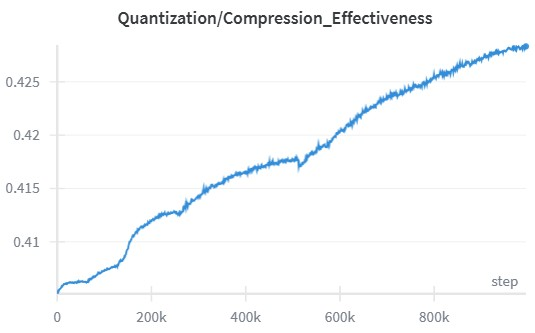
\includegraphics[width=0.75\linewidth]{../BabyLM_new/FIG/quantization.jpg}
    \caption{\textbf{Quantization effectiveness over training.} $E_q$ (fraction of ternary weights set to zero) stabilizes at 42.8\%, demonstrating efficient compression without downstream performance degradation.}
    \label{fig:bitmar_quant}
\end{figure}

\begin{figure}[!htb]
    \centering
    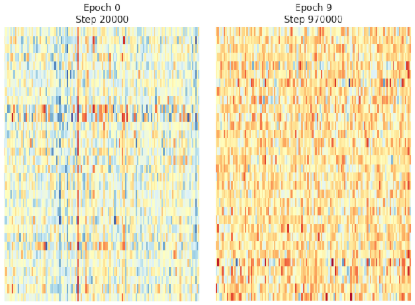
\includegraphics[width=\textwidth]{../BabyLM_new/FIG/BitMar-HeatMapComparisons.png}
    \caption{\textbf{Episodic memory slot activation patterns across training checkpoints.} Each row corresponds to a different checkpoint, ranging from early training (top, Epoch 0, step 20k) to late training (bottom, Epoch 9, step 97k). Early checkpoints show scattered, weak activations with minimal slot specialization. By the final checkpoint, memory slots develop strongly differentiated activation profiles, with specific slots specializing for distinct semantic categories. This convergence confirms that the episodic memory organizes stored representations by semantic content rather than recency.}
    \label{fig:bitmar_heatmap}
\end{figure}

\section{Experimental Results}
\label{sec:bitmar_results}

\subsection{Language Understanding Benchmarks}

\begin{table}[htbp]
\centering
\caption{\textbf{Language understanding benchmark performance.} \checkmark = natively 1-bit trained. Scores are accuracy (\%). WG = WinoGrande, CQA = CommonsenseQA, ARC-E = ARC-Easy.}
\label{tab:bitmar_lm_benchmarks}
\resizebox{\textwidth}{!}{%
\begin{tabular}{lcccccccc}
\toprule
\textbf{Model} & \textbf{Params} & \textbf{1-bit} & \textbf{ARC-E} & \textbf{BoolQ} & \textbf{HSwag} & \textbf{WG} & \textbf{CQA} & \textbf{MMLU} \\
\midrule
Bonsai 0.5B        & 500M & \checkmark & 58.25 & 58.44 & 48.01 & 54.46 & 18.43 & 25.74 \\
OLMo-BitNet 1B     & 1B   & \checkmark & 25.38 & 52.48 & 25.88 & 51.54 & 19.49 & 25.47 \\
Falcon3-1.58bit 7B & 7B   & $\times$   & 65.03 & 72.14 & 59.46 & 60.14 & 67.08 & 42.79 \\
LLaMA3-8B-1.58     & 8B   & $\times$   & 70.71 & 68.38 & 68.56 & 60.93 & 28.50 & 35.04 \\
BitNet b1.58 2B    & 2B   & \checkmark & 74.79 & 80.18 & 68.44 & 71.90 & 71.58 & 53.17 \\
\midrule
\textbf{BitMar-14M (Ours)} & 14M & \checkmark & 28.32 & \textbf{42.83} & 30.04 & \textbf{54.57} & 24.57 & 27.90 \\
\bottomrule
\end{tabular}%
}
\end{table}

Table~\ref{tab:bitmar_lm_benchmarks} compares BitMar-14M against low-bit quantized baselines. Despite being 35$\times$ smaller than the next-smallest baseline (Bonsai 0.5B), BitMar achieves competitive BoolQ (42.83\%) and WinoGrande (54.57\%), demonstrating strength in binary reasoning and coreference. ARC-Easy (28.32\%) and HellaSwag (30.04\%) trail larger models, reflecting capacity limits on multi-step commonsense reasoning.

\subsection{BabyLM Evaluation Suite}

\begin{table}[htbp]
\centering
\caption{\textbf{BitMar BabyLM evaluation.} Average finetuned NLP accuracy: 60.5\%.}
\label{tab:bitmar_babylm}
\begin{tabular}{llll}
\toprule
\textbf{Category} & \textbf{Task} & \textbf{Metric} & \textbf{Score} \\
\midrule
\multirow{7}{*}{Finetune NLP} & BoolQ & Accuracy & 66.5\% \\
 & MNLI & Accuracy & 42.3\% \\
 & MRPC & Accuracy & 69.1\% \\
 & MultiRC & Accuracy & 57.6\% \\
 & QQP & Accuracy & 70.2\% \\
 & RTE & Accuracy & 54.0\% \\
 & WSC & Accuracy & 63.5\% \\
\midrule
\multirow{3}{*}{Multimodal} & DevBench & Visual Vocab Acc. & 21.2\% \\
 & VQA & Accuracy & 21.4\% \\
 & Winoground & Accuracy & 23.8\% \\
\midrule
World Knowledge & EWoK & Accuracy & 24.9\% \\
\midrule
\multirow{3}{*}{Linguistic} & BLiMP & Accuracy & 48.7\% \\
 & Compositional & Accuracy & 51.5\% \\
 & Entity Tracking & Accuracy & 31.2\% \\
\midrule
Psycholinguistic & Reading Comp. & Score & 0.44 \\
\midrule
\multirow{2}{*}{Morphology} & Wug Adj. & Correlation & $-$0.16 \\
 & Wug Past & Correlation & $-$0.22 \\
\bottomrule
\end{tabular}
\end{table}

BitMar achieves 60.5\% average across finetuned NLP benchmarks, with strengths in paraphrase detection (QQP: 70.2\%, MRPC: 69.1\%) and reading comprehension (BoolQ: 66.5\%). Multimodal tasks score 21--25\%, with the highest result on EWoK (24.9\%), plausibly due to episodic memory providing relevant context. Negative Wug morphology correlations ($-$0.16, $-$0.22) indicate systematic limits in morphological productivity under extreme compression.

\subsection{Episodic Memory Ablation}

\begin{table}[htbp]
\centering
\caption{\textbf{Inference efficiency with and without episodic memory.}}
\label{tab:bitmar_eff_ablation}
\begin{tabular}{lcc}
\toprule
\textbf{Metric} & \textbf{Memory On} & \textbf{Memory Off} \\
\midrule
Throughput (tok/s) & \textbf{57.3} & 7.7 \\
Latency/token (ms) & \textbf{17.3} & 129.8 \\
Energy (J) & \textbf{1.90} & 9.17 \\
RAM (MB) & \textbf{956} & 1{,}076 \\
\bottomrule
\end{tabular}
\end{table}

\begin{table}[htbp]
\centering
\caption{\textbf{Zero-shot accuracy deltas ($\Delta$ pp) with episodic memory enabled.}}
\label{tab:bitmar_acc_ablation}
\begin{tabular}{lc}
\toprule
\textbf{Task} & \textbf{$\Delta$ (pp)} \\
\midrule
Entity Tracking (Split 1) & +2.9 \\
Entity Tracking (Split 2) & +4.1 \\
COMPS & +3.4 \\
BLiMP & +0.6 \\
VQA & +3.4 \\
EWoK (Split 1) & $-$1.6 \\
EWoK (Split 2) & +1.0 \\
Winoground & $-$1.6 \\
DevBench & No effect \\
\bottomrule
\end{tabular}
\end{table}

Episodic memory provides 7.5$\times$ throughput improvement, 79\% energy reduction, and 11\% lower RAM usage. Zero-shot accuracy gains of 3--4 pp are consistent across entity tracking and visual question answering. Two regressions (Winoground $-$1.6pp, EWoK Split 1 $-$1.6pp) are attributed to the fixed-capacity memory occasionally introducing irrelevant context, a tradeoff inherent in any fixed-size retrieval system.

\section{Implementation Details}
\label{sec:bitmar_impl}

\subsection{Hyperparameters}

Table~\ref{tab:bitmar_arch_hyperparams} lists the architectural hyperparameters and Table~\ref{tab:bitmar_train_hyperparams} lists the training configuration.

\begin{longtable}{lp{6cm}}
\caption{\textbf{BitMar architectural hyperparameters.} Full specification of the 14M-parameter ternary-quantized architecture.}
\label{tab:bitmar_arch_hyperparams} \\
\toprule
\textbf{Hyperparameter} & \textbf{Value} \\
\midrule
\endfirsthead
\multicolumn{2}{c}{\tablename\ \thetable{} (continued)} \\
\toprule
\textbf{Hyperparameter} & \textbf{Value} \\
\midrule
\endhead
\midrule
\multicolumn{2}{r}{\textit{Continued on next page}} \\
\endfoot
\bottomrule
\endlastfoot
\multicolumn{2}{l}{\textit{Text Encoder}} \\
\quad Transformer layers & 4 \\
\quad Hidden dimension $d$ & 128 \\
\quad Attention heads $h$ & 4 \\
\quad Max sequence length & 256 tokens \\
\quad Weight quantization & Ternary $\{-1,0,+1\}$, learned per-layer scale \\
\quad Activation quantization & Per-token 8-bit max-abs, range $[-127,127]$ \\
\quad Attention sinks $S$ & 4 \\
\quad Sliding window $W$ & 1{,}020 \\
\midrule
\multicolumn{2}{l}{\textit{Vision Encoder}} \\
\quad Vision backbone & DiNOv2 (frozen, offline feature extraction) \\
\quad DiNOv2 feature dimension & 768 \\
\quad Spatial pooling & $2\times2$ average pooling \\
\quad MLP compression $\mathbf{W}_1$ & $\mathbb{R}^{384\times768}$ \\
\quad MLP compression $\mathbf{W}_2$ & $\mathbb{R}^{128\times384}$ \\
\quad Output dimension & 128 \\
\midrule
\multicolumn{2}{l}{\textit{Cross-Modal Fusion}} \\
\quad Fusion type & Cross-attention (text queries, vision K/V) \\
\quad Projection quantization & 1.58-bit ternary \\
\quad Fusion output & $\mathbf{F} \in \mathbb{R}^{n_t \times 128}$ \\
\quad Memory query pooling & Mean pooling $\rightarrow \mathbf{q}_{\text{mem}} \in \mathbb{R}^{128}$ \\
\midrule
\multicolumn{2}{l}{\textit{Episodic Memory}} \\
\quad Memory slots $K$ & 512 \\
\quad Memory dimension $C$ & 128 \\
\quad Write rate $\alpha$ & 0.2 \\
\quad Memory regularization $\lambda$ & 0.1 \\
\quad Addressing mechanism & Content-based (softmax inner product) \\
\midrule
\multicolumn{2}{l}{\textit{Decoder}} \\
\quad Transformer layers & 4 \\
\quad Hidden dimension & 128 \\
\quad Attention heads & 4 \\
\quad Max generation length & 256 tokens \\
\quad Attention sinks & Same as encoder \\
\quad Output vocabulary & GPT-2 BPE (50{,}257 tokens) \\
\quad Output projection & Ternary weights, FP32 logits \\
\end{longtable}

\begin{table}[htbp]
\centering
\caption{\textbf{BitMar training hyperparameters.} Optimizer, schedule, memory, and hardware settings used across the full 10-epoch run.}
\label{tab:bitmar_train_hyperparams}
\begin{tabular}{lp{5.5cm}}
\toprule
\textbf{Hyperparameter} & \textbf{Value} \\
\midrule
\multicolumn{2}{l}{\textit{Training}} \\
\quad Optimizer & AdamW8bit \\
\quad Learning rate & $2 \times 10^{-4}$ \\
\quad Cosine restart $T_0$ & 1{,}000 steps \\
\quad Cosine restart $T_{\text{mult}}$ & 2 \\
\quad Min learning rate $\eta_{\min}$ & $0.1 \times \text{lr}$ \\
\quad Effective batch size & 128 \\
\quad Training epochs & 10 \\
\quad Precision & FP16 \\
\quad Gradient checkpointing & Yes \\
\quad Training hardware & NVIDIA A6000 \\
\midrule
\multicolumn{2}{l}{\textit{Loss Weights}} \\
\quad Language modeling $\mathcal{L}_{\text{lm}}$ & 1.0 \\
\quad Cross-modal contrastive $\mathcal{L}_{\text{cm}}$ & 1.5 \\
\quad Memory consistency $\mathcal{L}_{\text{mem}}$ & 0.1 \\
\midrule
\multicolumn{2}{l}{\textit{Adaptive Training Controller}} \\
\quad EMA window & 200 steps \\
\quad Drop threshold & 0.12 \\
\quad Freeze/boost duration & 1{,}500 steps \\
\quad Min intervention interval & 800 steps \\
\bottomrule
\end{tabular}
\end{table}

\subsection{Training Corpus}

Table~\ref{tab:bitmar_dataset_stats} details the composition of BitMar's 101M-token training corpus. Multimodal pairs (50M tokens) from CC3M and Localized Narratives provide visual-language grounding; text-only data (50M tokens) from six sources provides linguistic coverage. A 1M-token stratified hold-out set is reserved for evaluation.

\begin{table}[htbp]
\centering
\caption{\textbf{BitMar training corpus composition.} The 101M-token corpus combines 50M multimodal tokens and 50M text-only tokens, with a 1M-token stratified hold-out set.}
\label{tab:bitmar_dataset_stats}
\begin{tabular}{llr}
\toprule
\textbf{Type} & \textbf{Source} & \textbf{Tokens} \\
\midrule
\multirow{2}{*}{Multimodal (50M)} & CC3M (Conceptual Captions) & $\sim$28M \\
 & Localized Narratives & $\sim$22M \\
\midrule
\multirow{6}{*}{Text-only (50M)} & BNC Spoken & $\sim$10M \\
 & CHILDES & $\sim$5M \\
 & Gutenberg & $\sim$12M \\
 & OpenSubtitles & $\sim$10M \\
 & Simple English Wikipedia & $\sim$5M \\
 & Switchboard & $\sim$8M \\
\midrule
Hold-out & Mixed (stratified) & 1M \\
\midrule
\textbf{Total} & & \textbf{101M} \\
\bottomrule
\end{tabular}
\end{table}

\subsection{Tokenizer and Preprocessing}

BitMar uses the GPT-2 Byte Pair Encoding (BPE) tokenizer with a vocabulary size of 50{,}257 tokens. Text sequences exceeding 256 tokens are truncated; shorter sequences are padded. DiNOv2 visual features are extracted offline using a frozen DiNOv2 (large) backbone, storing $2\times2$-pooled 768-dimensional patch features as memory-mapped \texttt{.npy} files. During training, features are loaded with on-the-fly compression to reduce I/O overhead. Each multimodal sample is an (image, caption) pair, with the caption tokenized using the GPT-2 BPE tokenizer.

\subsection{External Memory Offloading}

For memory-constrained devices, the memory matrix $\mathbf{M}$ can be offloaded to external storage via a utility that saves and loads memory tensors without gradient tracking. This preserves the persistent memory state between sessions without increasing runtime RAM usage. The offload is triggered automatically when device RAM drops below a configurable threshold, making BitMar deployable on hardware with as little as 512~MB RAM.

\section{Lessons Learned and Research Directions}
\label{sec:bitmar_lessons}

BitMar validates three design hypotheses that directly motivated EmberVLM:

\paragraph{Validated: episodic memory is compatible with and beneficial for quantized multimodal models.} The efficiency gains and accuracy improvements confirm that episodic memory can replace heavy long-range attention even under aggressive 1.58-bit quantization.

\paragraph{Validated: 1.58-bit quantization is compatible with cross-modal fusion.} BabyLM multimodal task performance demonstrates that ternary weights support meaningful cross-modal alignment at 14M parameters.

\paragraph{Open: Can episodic memory address hallucination?} BitMar's memory improves coherence but has no mechanism for detecting visually ungrounded tokens. This gap directly motivated the Visual Absence Refiner in EmberVLM (Section~\ref{sec:embervlm_refiner}).

\paragraph{Open: Can the architecture scale to mission-critical classification?} BitMar's evaluation is primarily generative. Whether memory-augmented tiny VLMs can achieve reliable multi-label classification in safety-critical settings required a dedicated training pipeline and evaluation framework: the EmberVLM design.

\paragraph{Open: Can memory be truly adaptive at deployment?} BitMar's memory is essentially static at deployment: slots do not update after training. EmberVLM's novelty-triggered online writes (Section~\ref{sec:memory_novelty}) directly address this gap.
